% Charlotte Geiger - Manuel Lippert - Leonard Schatt
% Physikalisches Praktikum

% Teilauswertung X

\section{Umkehrdifferenzierer}
\subsection*{Vergleich der optimierten mit der nicht optimierten Schaltung}
Im folgenden wird diskutiert, inwiefern sich die Ausgangsspannung des Umkehrdifferenzierers ändert, wenn man die Grundschaltung aus Abbildung \ref{Differenzierschaltung} verwendet, 
oder wenn man Schaltung  verwendet.

\begin{center}
    \begin{figure}
        \centering
        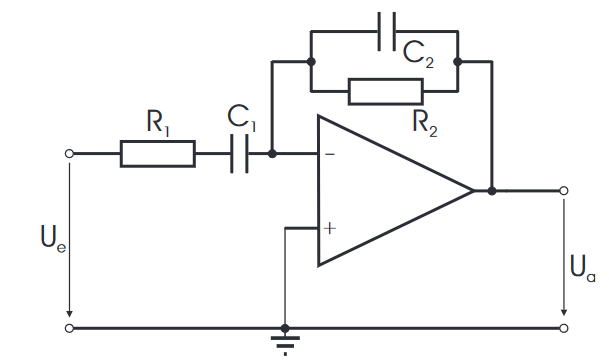
\includegraphics[width = 8cm]{diffOPV_verbessert.PNG}
        \caption{Modifizierte Version eines Umkehrdifferenzierers}
        \label{modifiziertumkehrdiff}
    \end{figure}
\end{center} 
 
Wenn man das "differenzierte"  Bild der einfachen Schaltung \ref{Differenzierschaltung} betrachtet fällt einem sehr schnell auf, dass man einen Einschwingprozess wie in Grafik 
\ref{Einschwingprozess} beobachten kann. Dieser kommt daher, das die Schaltung nicht alles differenziert\footnotemark in dem Moment, in dem sich die Steigung sprunghaft ändert. 
Der Grund dafür ist, dass kein Wiederstand dem Kondensator $C_1$ vorgeschaltet ist. Bei hoher Frequenz ist der Widerstand des Kondensators sehr gering. Da der Innenwiderstand 
der Stromquelle nicht Null ist, fallen auch Teile der Spannung dort ab. 
\footnotetext{\url{file:///C:/Users/STUDIE~1/AppData/Local/Temp/Beschreibung%20Operationsverstarker.pdf}} 
Ein Teil des Signales wird undifferenziert durchgelassen. Dabei scheint dieser Prozess nicht bei allen Frequenzen im gleichen Maß abzulaufen. 
Man sieht, dass Eingangssignal von dem Funktionsgenerator erzeugt wird, eine komposition aus vielen Sinusspannungen zu sein scheint. Genauerer Informationen sollte man 
erhalten, wenn man das Ausgangssignal fouriertransformiert. 
Außerdem fällt auf, dass das Rauschen bei der Grundschaltung deutlich stärker ist, als bei der optimierten Schaltung.\\

\begin{figure}[h]
    \centering
    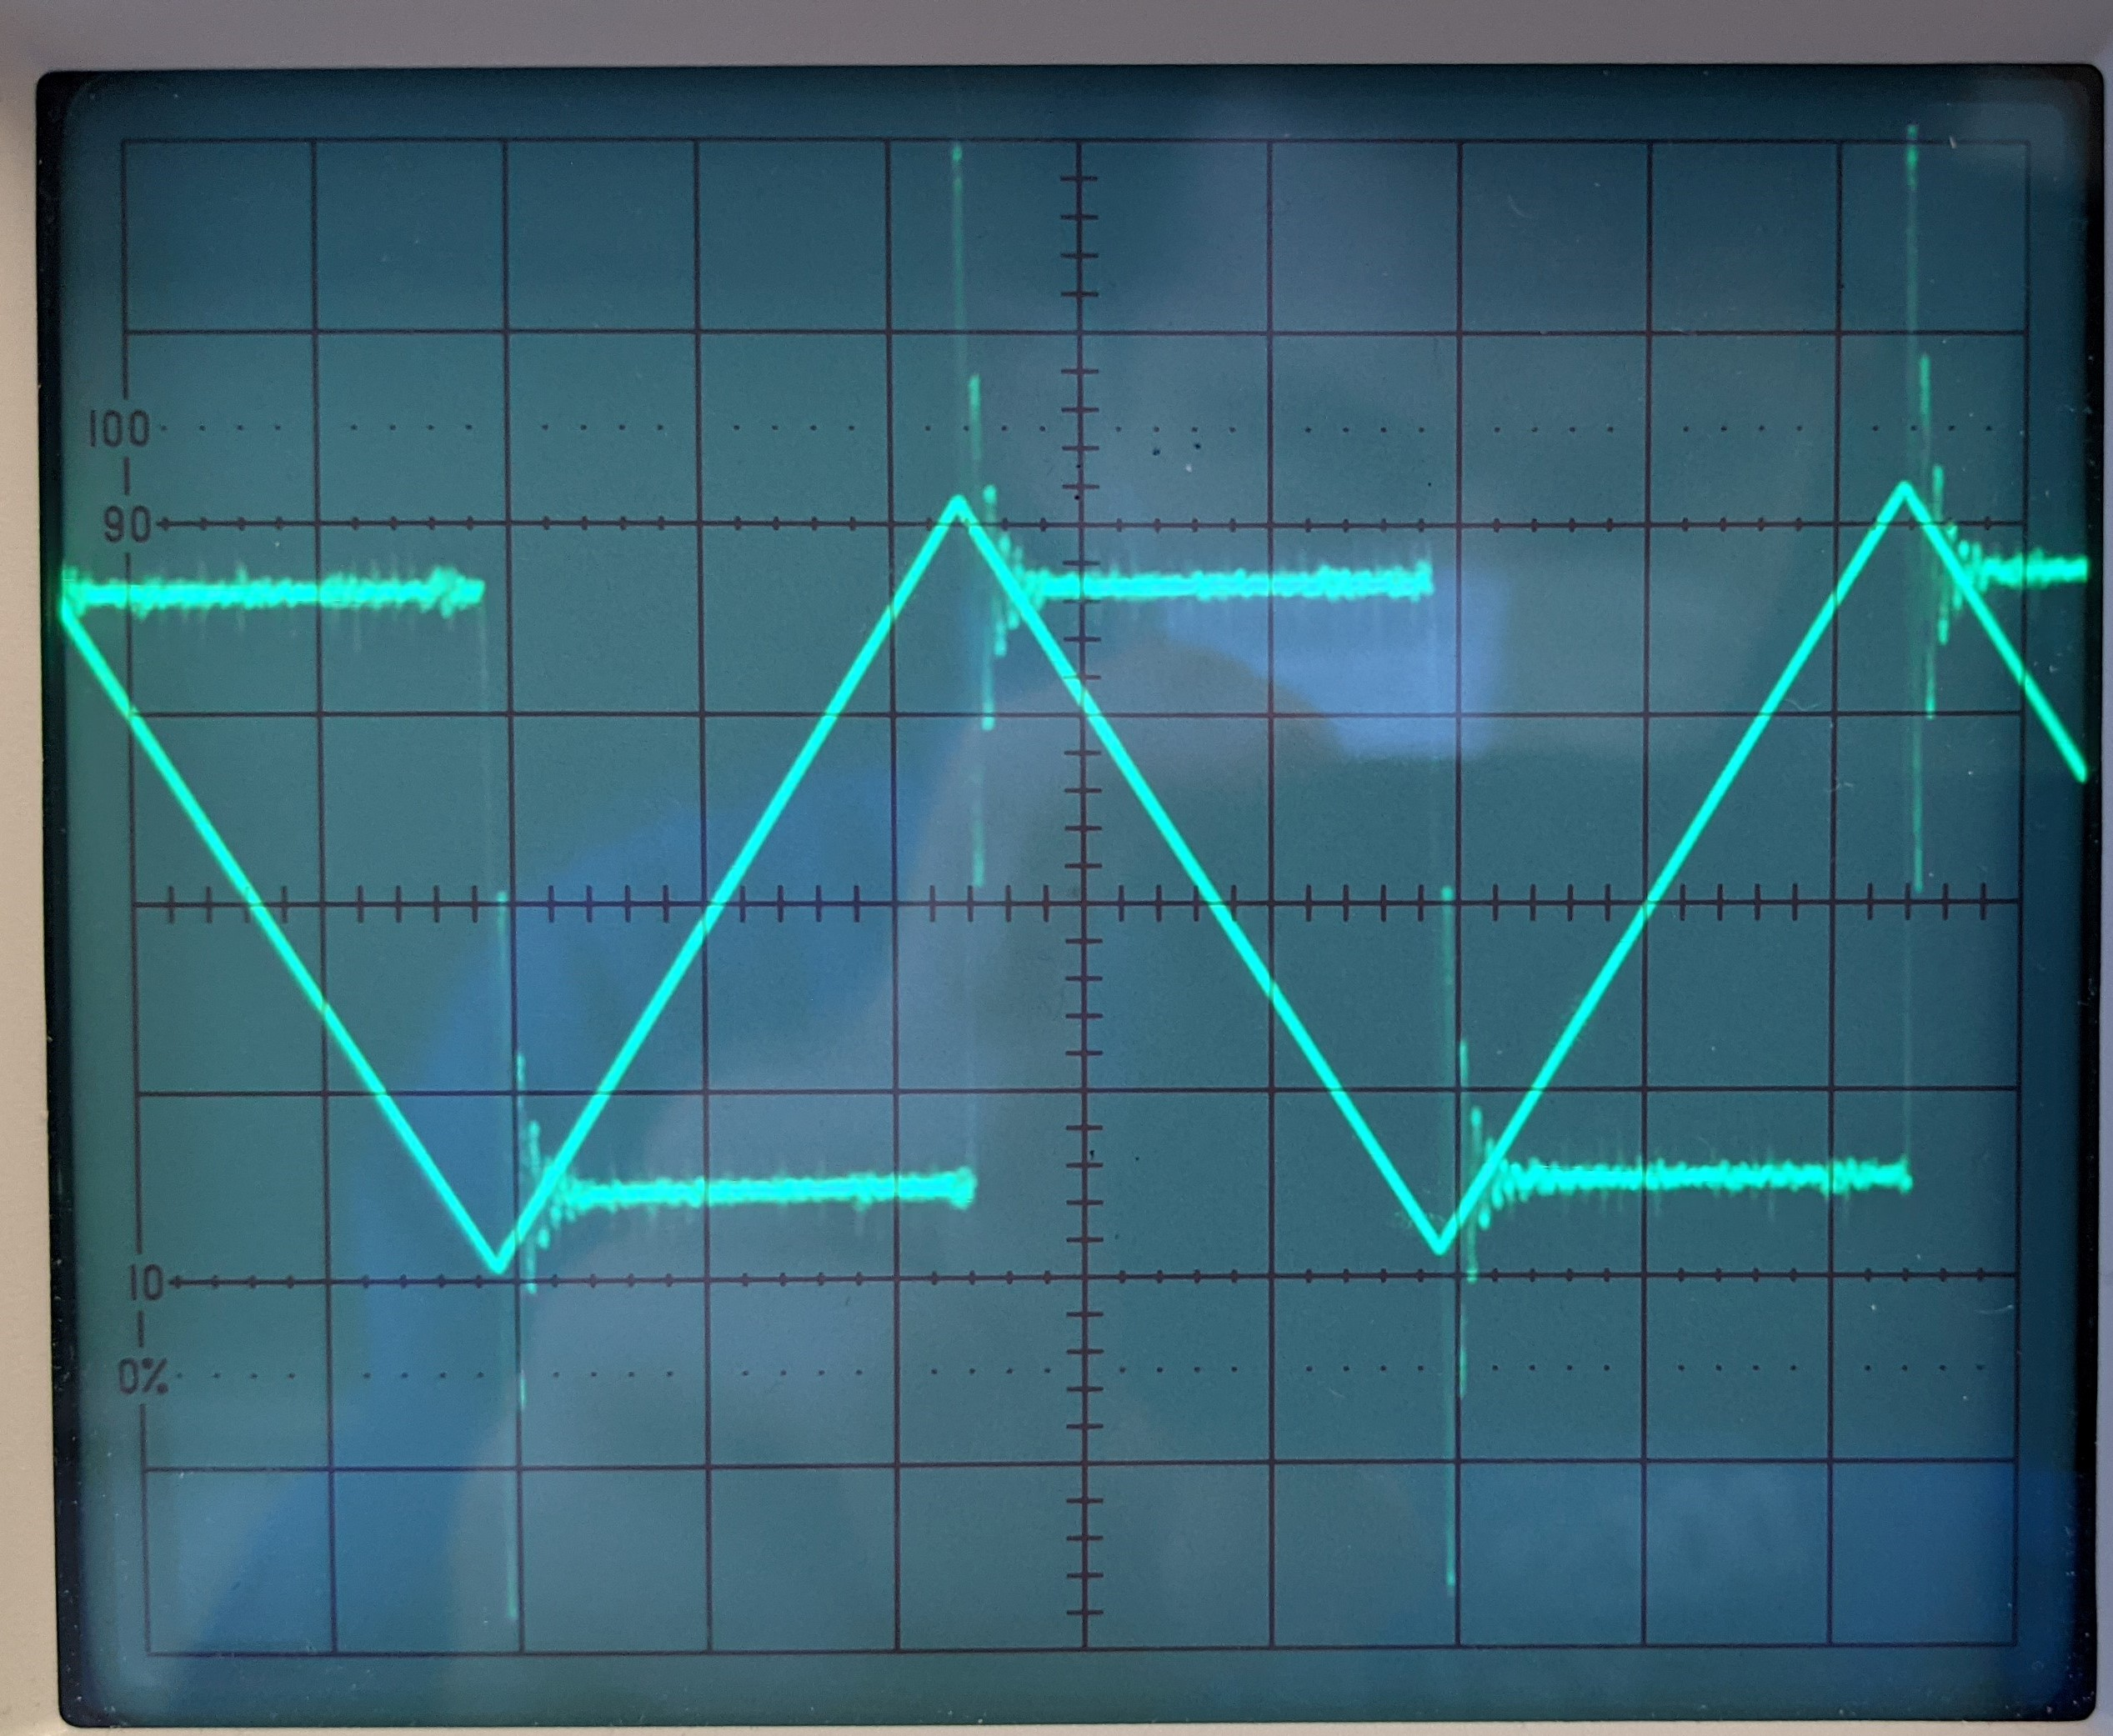
\includegraphics[width = 9cm]{Bilder/43-diffSchwingung.jpg}
    \caption{Einschwingprozess eines Umkehrdifferenzierers bei einer Dreiecksspannung mit der Frequnenz $f$ = 1kHz }
    \label{Einschwingprozess}
\end{figure}

Betrachten wir nun, dass die Ausgangssignal der modifizierten Schaltung aus Abbildung \ref{modifiziertumkehrdiff}. Dabei würden 
wir erwarten, dass das Rauschen stark vermindert wird, weil der Kondensator $C_2$ wie ein Teifpassfilter einfluss nimmt. Damit filtert er auch 
das Einschwingen sehr gut weg. Es bleibt der Gleichstromanteil in der Spannung.
\begin{figure}[h]
    \centering
    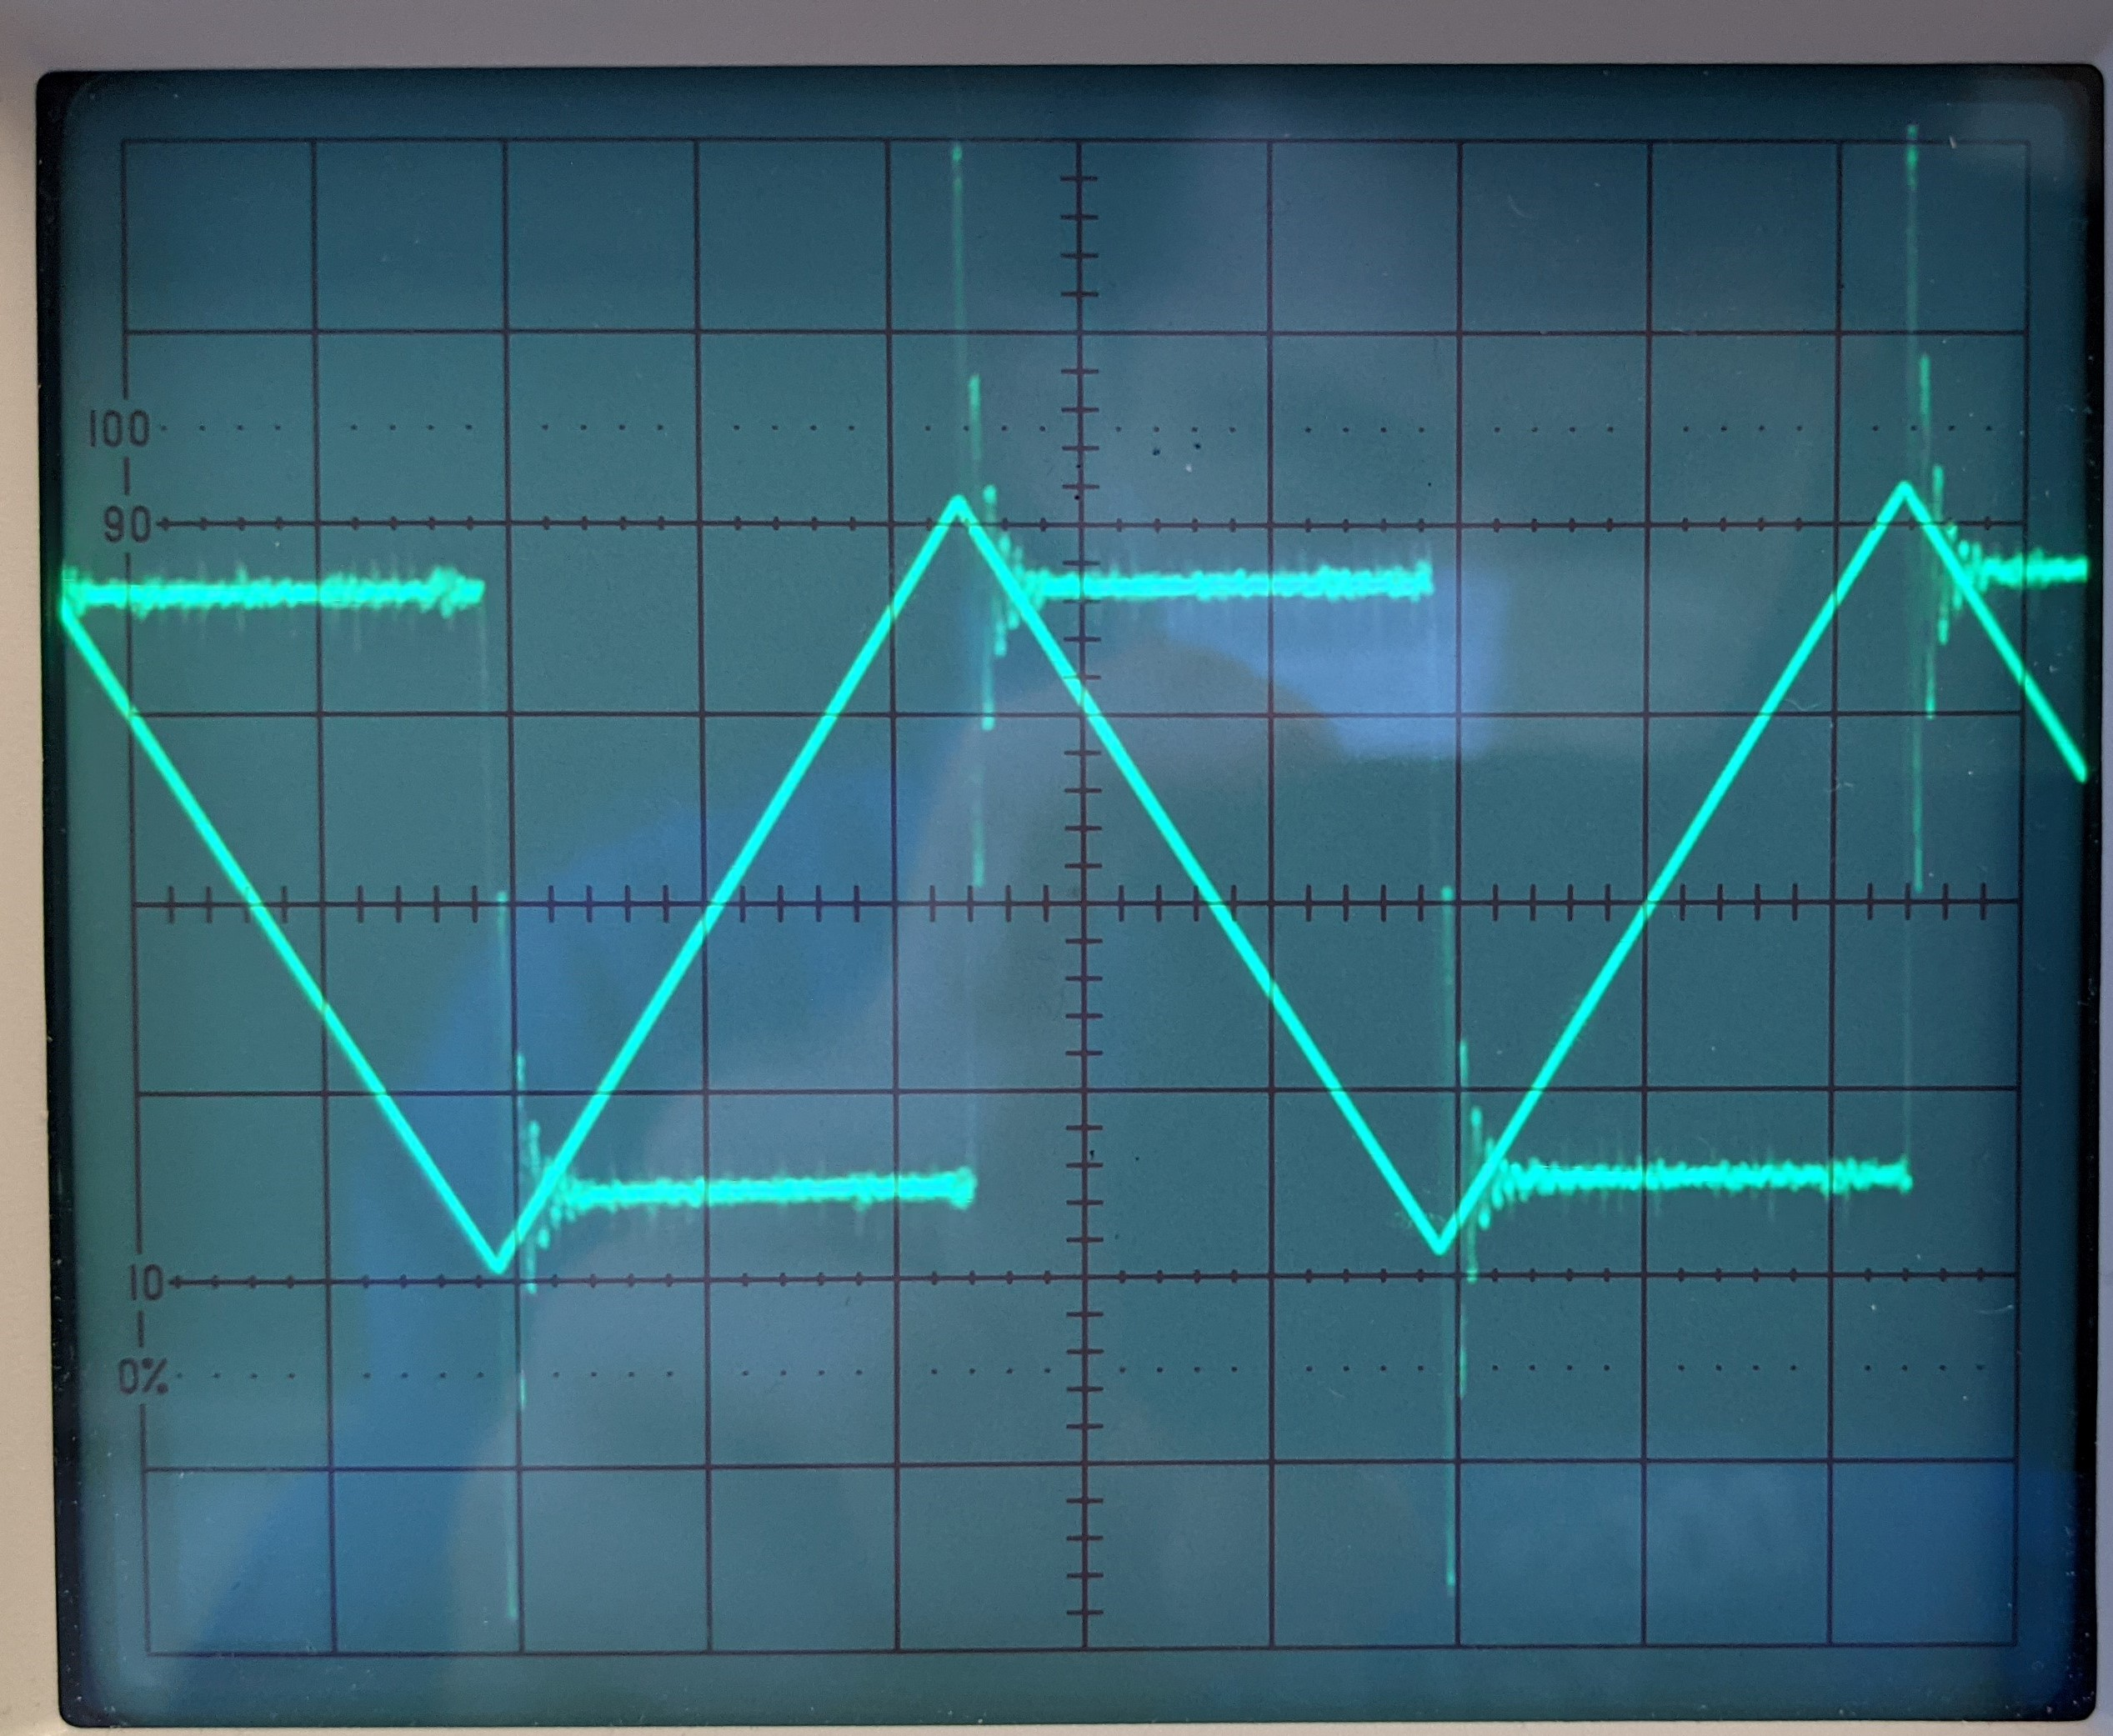
\includegraphics[width = 9cm]{Bilder/43-diffSchwingung.jpg}
    \caption{Einschwingprozess eines Umkehrdifferenzierers bei einer Dreiecksspannung mit der Frequenz $f$ = 1kHz }
    \label{Einschwingprozess}
\end{figure}
Das Differenzieren ist nicht perfekt, wegen der endlichen Flankenabfallzeit. Diese ist auf das Auf- und Entladen des Kondensators.
\section*{Zusammenhang zwischen dem Frequenzgang des Umkehrintegrators und dem des Umkehrdifferenzierers}
